\documentclass[12pt]{article}
\usepackage[utf8]{inputenc}
\usepackage[greek,english]{babel}
\usepackage{alphabeta}
\usepackage{fancyhdr}
\usepackage{listings}
\usepackage{mathtools}
\usepackage{xcolor}
\usepackage{float}
\usepackage{tabularx}
\usepackage[margin=0.5in]{geometry}
\usepackage[backend=bibtex]{biblatex}
\usepackage{hyperref}
\hypersetup{
	colorlinks=true,
	linktoc=all,
	linkcolor=black,
}
\title{Εργασία Τεχνολογίας Λογισμικού -- Μέρος 3ο}
\author{Αντώνης Θωμάκος - 18390037 \\
Χρήστος Μαργιώλης - 19390133 \\
Στέφανος Στράους - 19390221}
\date{Μάιος 2022}

\begin{document}

\begin{titlepage}
        \maketitle
        \begin{figure}[t!]
        \begin{center}
        
\includegraphics[scale=1.0]{./res/uniwa-logo.pdf} \\
        \Large
        \textbf{Πανεπιστήμιο Δυτικής Αττικής} \\
        \large
        Τμήμα Μηχανικών Πληροφορικής και Ηλεκτρονικών Υπολογιστών
        \end{center}
        \end{figure}
\end{titlepage}

\renewcommand{\contentsname}{Περιεχόμενα}
\tableofcontents
\pagebreak

\section{Δομή φακέλων}

Ο φάκελος \lstinline{changes_to_previous_parts} περιέχει αλλαγές που αφορούν
προηγούμενα μέρη. Ο \lstinline{src} περιέχει τον πηγαίο κώδικα Java. Ο
\lstinline{doc} περιέχει τα αρχεία \LaTeX και τις εικόνες που χρησιμοποιήθηκαν
για την συγγραφή του παραδοτέου. Ο \lstinline{executable} περιέχει τα
εκτελέσιμα αρχεία για τους πηγαίους κώδικες.

\section{Διάγραμμα κλάσεων για όλο το Π.Σ}

\begin{figure}[H]
	\centering
	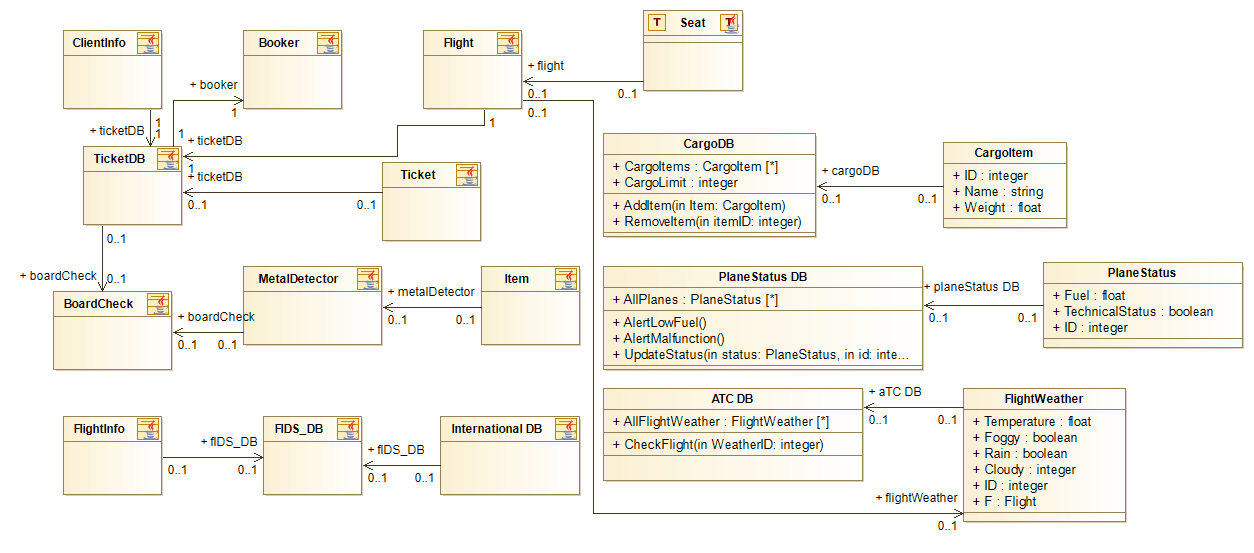
\includegraphics[width=\linewidth]{./res/AllClasses.png}
\end{figure}

\section{Διάγραμμα κλάσεων για τις περιπτώσεις χρήσης}

\subsection{Περίπτωση χρήσης 1 -- Κράτηση εισιτηρίων}

\begin{figure}[H]
	\centering
	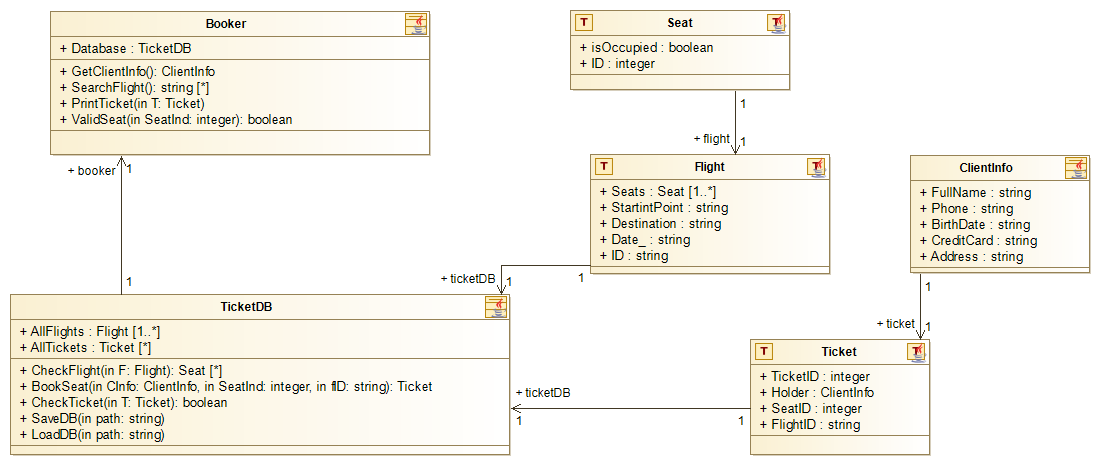
\includegraphics[width=\linewidth]{./res/UC1_Impl.png}
\end{figure}

\subsection{Περίπτωση χρήσης 2 -- 'Ελεγχος εγκυρότητας εισιτηρίων (Check In)}

\begin{figure}[H]
	\centering
	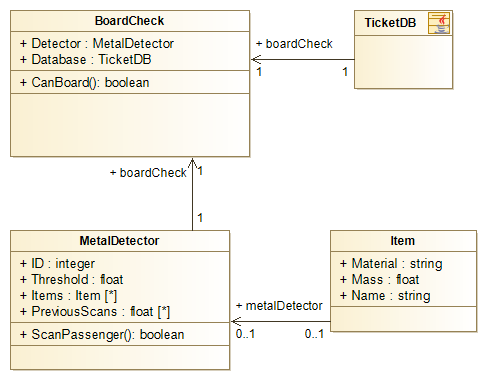
\includegraphics[width=\linewidth]{./res/UC2_Impl.png}
\end{figure}

\subsection{Περίπτωση χρήσης 3 -- Πληροφορίες πτήσεις (F.I.D.S)}

\begin{figure}[H]
	\centering
	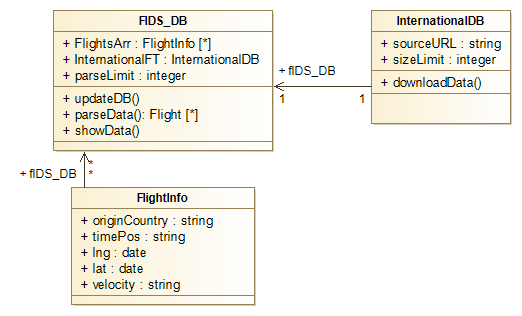
\includegraphics[width=\linewidth]{./res/UC3_Impl.png}
\end{figure}

\section{Περιπτώσης δοκιμής}

\subsection{Περίπτωση δοκιμής 1 -- Κράτηση εισιτηρίων}

\begin{center}
\begin{tabular}{|p{5cm}|p{12cm}|}
	\hline
	\textbf{Απαιτήσεις} &
	Να κάνει κράτηση εισιτηρίου ο χρήστης και να αποθηκευτεί στην βάση
	δεδομένων. \\
	\hline
	\textbf{Περιγραφή δοκιμής} &
	Ο χρήστης εισάγει τα στοιχεία του και επιχειρεί να κλείσει μία θέση για
	μία επιθυμητή πτήση. \\
	\hline
	\textbf{Δοκιμαστικά δεδομένα} &
	Πέντε προκαθορισμένες πτήσεις μέσα στην βάση δεδομένων. \\
	\hline
	\textbf{Αναμενόμενα αποτέλεσματα} &
	Μέτα το τέλος της δοκιμής τυπώνεται το εισιτήριο του χρήστη και
	αποθηκεύεται σε αρχείο της βάσης δεδομένων. \\
	\hline
	\textbf{Συνθήκες δοκιμής -- Διαμόρφωση συστήματος} &
	Να υπάρχει πρόσβαση στο φάκελο με τη βάση δεδομένων. \\
	\hline
	\textbf{Βηματικές οδηγίες -- Διαδικασίες δοκιμής} &
	\begin{itemize}
		\item Ο χρήστης εισάγει τα στοιχεία του.
		\item Το Π.Σ αποκρίνεται δείχνοντας διαθέσιμες πτήσεις.
		\item Ο χρήστης επιλέγει την επιθυμητή πτήση.
		\item Το σύστημα αποκρίνεται δείχνοντας διαθέσιμες θέσεις (αν
			υπάρχουν).
		\item Ο χρήστης επιλέγει την επιθυμητή θέση.
		\item Το Π.Σ τυπώνει το εισιτήριο και το αποθηκεύει στην βάση
			δεδομένων.
	\end{itemize} \\
	\hline
	\textbf{Μετά την εκτέλεση της δοκιμής} &
	\begin{tabularx}{12cm}{X|X}
		\textbf{Πέρασε τη δοκιμή} & \textbf{Αναλυτικά αποτελέσματα δοκιμής} \\ 
		\hline
		Ναι. & Το Π.Σ έσωσε με επιτυχία το αρχείο της βάσης δεδομένων
		και τύπωσε κανονικά το εισιτήριο του χρήστη. \\
	\end{tabularx} \\
	\hline
\end{tabular}
\end{center}
\pagebreak

\subsection{Περίπτωση δοκιμής 2 -- 'Ελεγχος εγκυρότητας εισιτηρίων (Check in)}

\begin{center}
\begin{tabular}{|p{5cm}|p{12cm}|}
	\hline
	\textbf{Απαιτήσεις} &
	'Ελεγχος ότι ο επιβάτης δεν μπορεί να επιβιβαστεί αν δώσει άκυρο
	εισιτήριο ή έχει απαγορευμένα αντικείμενα. \\
	\hline
	\textbf{Περιγραφή δοκιμής} &
	Ο χρήστης εισάγει άκυρο εισιτήριο, αλλά δεν έχει απαγορευμένα
	αντικείμενα και τα αντικείμενα είναι κάτω του όριο ανοχής του ανιχνευτή
	μετάλλων. \\
	\hline
	\textbf{Δοκιμαστικά δεδομένα} &
	Στο Π.Σ είναι αποθηκευμένα τα δεδομένα που εντόπισε ο ανιχνευτής
	μετάλλων. \\
	\hline
	\textbf{Αναμενόμενα αποτέλεσματα} &
	Μετά το τέλος της περίπτωσης δοκιμής, ο χρήστης δεν μπορεί να
	επιβιβαστεί. \\
	\hline
	\textbf{Συνθήκες δοκιμής -- Διαμόρφωση συστήματος} &
	Να έχει πρόσβαση στην βάση δεδομένων των εισιτηρίων. \\
	\hline
	\textbf{Βηματικές οδηγίες -- Διαδικασίες δοκιμής} &
	\begin{itemize}
		\item Ο χρήστης εισάγει τα στοιχεία του εισιτηρίου του.
		\item Το Π.Σ αποκρίνεται ελέγχοντας τα στοιχεία του εισιτηρίου
			και τα αποτελέσματα του ανιχνευτή μετάλλων.
		\item Το Π.Σ αποκρίνεται ενημερώνοντας τον χρήστη ότι δεν
			μπορεί να επιβιβαστεί.
	\end{itemize} \\
	\hline
	\textbf{Μετά την εκτέλεση της δοκιμής} &
	\begin{tabularx}{12cm}{X|X}
		\textbf{Πέρασε τη δοκιμή} & \textbf{Αναλυτικά αποτελέσματα δοκιμής} \\ 
		\hline
		Ναι. & Το Π.Σ βρήκε ότι το εισιτήριο δεν υπάρχει στην βάση
		δεδομένων και δεν επέτρεψε την επιβίβαση. \\
	\end{tabularx} \\
	\hline
\end{tabular}
\end{center}
\pagebreak

\subsection{Περιπτωσή δοκιμής 3 -- Πληροφορίες πτήσεις (F.I.D.S)}

\begin{center}
\begin{tabular}{|p{5cm}|p{12cm}|}
	\hline
	\textbf{Απαιτήσεις} &
	Να εμφανίζονται στις οθόνες του αεροδρομίου οι πληροφορίες πτήσεων. \\
	\hline
	\textbf{Περιγραφή δοκιμής} &
	Το Π.Σ πρέπει να ενημερώνεται από βάση δεδομένων στο διαδίκτυο και να
	εμφανίζει τα δεδομένα των πτήσεων. \\
	\hline
	\textbf{Δοκιμαστικά δεδομένα} &
	Αρχείο πληροφοριών πτήσεων από το διαδίκτυο. \\
	\hline
	\textbf{Αναμενόμενα αποτέλεσματα} &
	Να εμφανίζονται οι πληροφορίες πτήσης. \\
	\hline
	\textbf{Συνθήκες δοκιμής -- Διαμόρφωση συστήματος} &
	Πρόσβαση στο διαδίκτυο. \\
	\hline
	\textbf{Βηματικές οδηγίες -- Διαδικασίες δοκιμής} &
	\begin{itemize}
		\item Το Π.Σ συνδέεται στην βάση δεδομένων και κατεβάζει τα
			δεδομένα.
		\item Το Π.Σ εμφανίζει τα δεδομένα των πτήσεων σε αναγνώσιμη
			μορφή.
	\end{itemize} \\
	\hline
	\textbf{Μετά την εκτέλεση της δοκιμής} &
	\begin{tabularx}{12cm}{X|X}
		\textbf{Πέρασε τη δοκιμή} & \textbf{Αναλυτικά αποτελέσματα δοκιμής} \\ 
		\hline
		Ναι. & Το Π.Σ εμφάνισε όλες τις πληροφορίες με επιτυχία. \\
	\end{tabularx} \\
	\hline
\end{tabular}
\end{center}
\pagebreak

\end{document}
